\documentclass[a4paper, 14pt]{extarticle}

\usepackage{xltxtra} % XeLaTex

\setromanfont{Liberation Sans} %Fonts setup
\setsansfont{Liberation Sans}
\setmonofont{DejaVu Sans Mono}

\usepackage{geometry}
\geometry{verbose,a4paper,tmargin=2cm,bmargin=2cm,lmargin=3.5cm,rmargin=1cm}

\usepackage{polyglossia} %Languages
\setmainlanguage{russian}
\setotherlanguage{english}

\PolyglossiaSetup{russian}{indentfirst=true} %Indentation
\parindent = 1cm

\usepackage{setspace}
\onehalfspacing
\hyphenpenalty=10000
\tolerance=1
\emergencystretch=1000

\usepackage{titlesec} %Настройка заголовков
\newcommand{\sectionbreak}{\clearpage}
\newcommand{\anonsection}[1]{\section*{#1}\addcontentsline{toc}{section}{#1}}
\newcommand{\anonsubsection}[1]{\subsection*{#1}\addcontentsline{toc}{subsection}{#1}}

\usepackage{enumitem} %Itemize customization

\usepackage[figurename=Рис.]{newfloat} %Floating environments
\usepackage{graphicx} %Images
\usepackage{pdfpages}
\DeclareGraphicsExtensions{.pdf,.png,.jpg}
\graphicspath{{images/pdf/}{images/png/}{images/jpg/}}

\usepackage[outputdir=\detokenize{../out/}, newfloat=true]{minted}
\setminted[cpp]{
linenos=true,
breaklines=true,
encoding=utf8,
frame=single,
fontsize=\small,
tabsize = 2
}
\makeatletter
\AtBeginEnvironment{minted}{\dontdofcolorbox}
\newcommand{\dontdofcolorbox{\renewcommand\fcolorbox[4][]{##4}}}{\xpatchcmd{\inputminted}{\minted@fvset}{\minted@fvset\dontdofcolorbox}{}{}}
\makeatother %Fix red box around cyrillic symbols in listings

\SetupFloatingEnvironment{listing}{name=Листинг}
\addto\captionsrussian{\renewcommand{\contentsname}{Оглавление}}

\usepackage{hyperref}
\usepackage[parentracker=true,
backend=biber,
hyperref=auto,
language=auto,
autolang=other,
citestyle=gost-numeric,
defernumbers=true,
bibstyle=gost-numeric,
]{biblatex}

% Russian sources first
\DeclareSourcemap{
\maps[datatype=bibtex]{
\map{
\step[fieldset=langid, fieldvalue={tempruorder}]
}
\map[overwrite]{
\step[fieldsource=langid, match=russian, final]
\step[fieldsource=presort, match=\regexp{(.+)}, replace=\regexp{aa$1}]  %$
}
\map{
\step[fieldsource=langid, match=russian, final]
\step[fieldset=presort, fieldvalue={az}]
}
\map[overwrite]{
\step[fieldsource=langid, notmatch=russian, final]
\step[fieldsource=presort, match=\regexp{(.+)}, replace=\regexp{za$1}]  %$
}
\map{
\step[fieldsource=langid, notmatch=russian, final]
}
\map{
\step[fieldsource=langid, match={tempruorder}, final]
\step[fieldset=langid, null]
}
}
}
%\xpatchbibmacro{related:default}
%  {\renewbibmacro*{pageref}{}}
%  {\renewbibmacro*{pageref}{}\renewbibmacro*{begentry}{}}{}{}
%\renewbibmacro*{begentry}
%  {\hspace{-4em}\makebox[4em]{\hyperlink{\thefield{entrykey}}{$\Downarrow$}}%
%       \raisebox{\baselineskip}{\hypertarget{back:\thefield{entrykey}}{}}}%
\edef\mytempforAtCharacter{\char64}
\def\getkey#1#2{%
\csappto{mytempforbibkey}{#1}%
\ifstrequal{#2}{,}
{\hspace{-4em}\makebox[4em]{\hyperlink{back:\mytempforbibkey}{$\Uparrow$}}%
\raisebox{\baselineskip}{\hypertarget{\mytempforbibkey}{}}%
\mytempforAtCharacter\mytempforbibtype\{\mytempforbibkey,}
{\getkey#2}%
}
\renewcommand*{\do}[1]{\csdef{#1}##1{\def\mytempforbibtype{#1}\def\mytempforbibkey{}\getkey}}
\docsvlist{MVBOOK,BOOK,INBOOK,SUPPBOOK,BOOKINBOOK,MVCOLLECTION,COLLECTION,INCOLLECTION,SUPPCOLLECTION,MVREFERENCE,REFERENCE,INREFERENCE,MVPROCEEDINGS,PROCEEDINGS,INPROCEEDINGS,PERIODICAL,ARTICLE,PATENT,ONLINE,THESIS,mvbook,book,inbook,suppbook,bookinbook,mvcollection,collection,incollection,suppcollection,mvreference,reference,inreference,mvproceedings,proceedings,inproceedings,periodical,article,patent,online,thesis,Article,Book,MVBook,InBook,BookInBook,SuppBook,Booklet,Collection,MVCollection,InCollection,SuppCollection,Manual,Misc,Online,Patent,Periodical,SuppPeriodical,Proceedings,MVProceedings,InProceedings,Reference,MVReference,InReference,Report,Thesis,Unpublished}
\renewcommand*{\do}[1]{\csdef{#1}##1{\mytempforAtCharacter #1\{}}
\docsvlist{XDATA,COMMENT,xdata,comment,}

\setcounter{biburllcpenalty}{7000}
\setcounter{biburlucpenalty}{8000}
\addbibresource{sources.bib}

\begin{document}

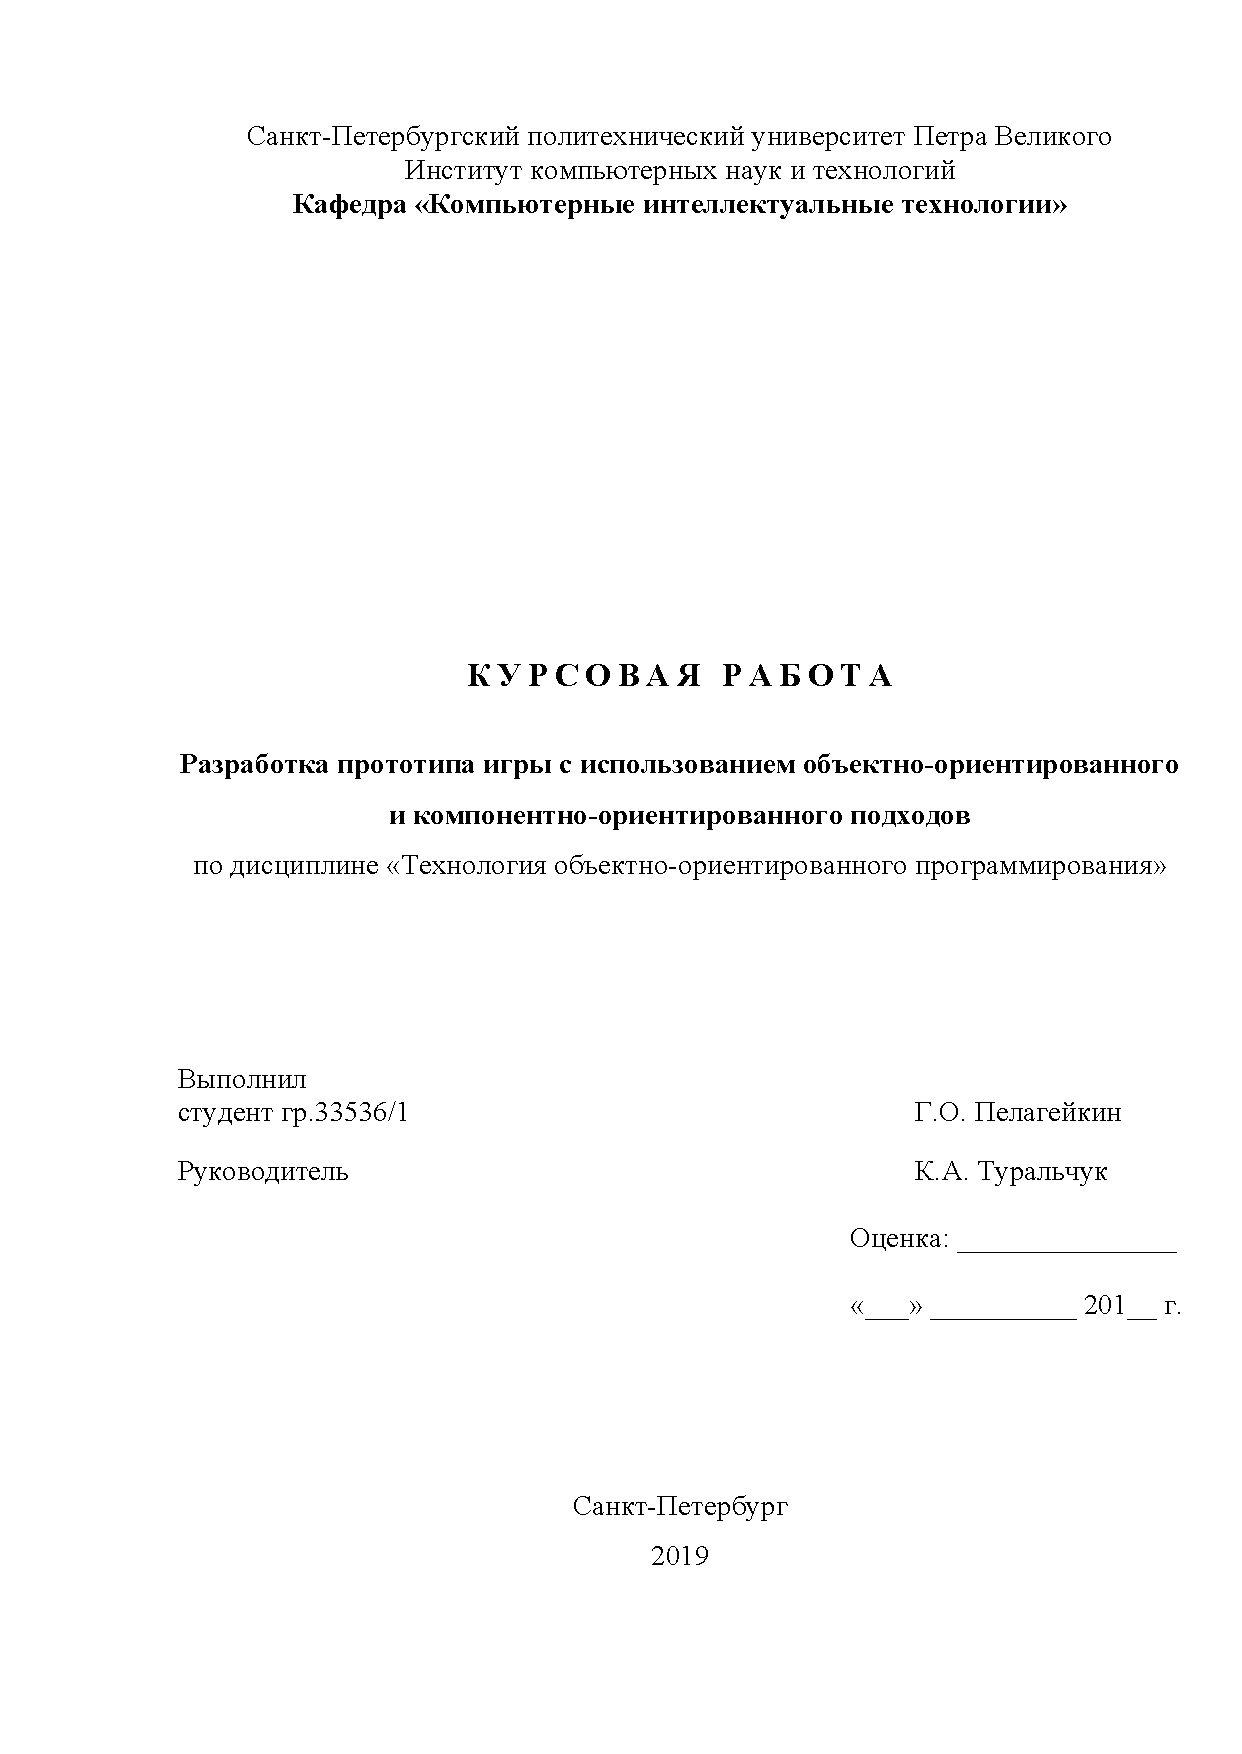
\includepdf{title-page}

\tableofcontents

\begin{anonsection}{Введение}
В данной работе будет рассмотрен процесс создания простой игры.
В качестве эталона была взята логика игры <<Atomic Bomber>>, реализация выполнена на языке C++ на основе легковесного игрового движка \verb|Urho3D|.
В ходе выполнения работы были выполнены следующие задачи:
\begin{enumerate}
\item Декомпозиция задачи.
\item Реализация основных компонентов игры с использованием парадигмы объектно-ориентированного программирование, а также компонентно-ориентированного подхода, средства реализации которого предоставлены движком \verb|Urho3D|.
\item Тестирование и отладка приложения.
\end{enumerate}

\end{anonsection}

\begin{section}{Постановка задачи}
Приведем основные аспекты игровой логики, которые будут реализованы.
В качестве эталона рассматривалась игровая логика <<Atomic Bomber>> за авторством Luke Allen:

\begin{enumerate}
\item Игровой мир двухмерный, вид сбоку.
\item Нижнюю часть экрана занимает случайно сгенерированный ландшафт, на поверхности которого могут находиться противники.
\item Игрок управляет самолетом, имеющим постоянную скорость.
Правая и левые стороны "закольцованы" друг на друга (т.е. пролет через них телепортирует игрока к противоположной границе), вылет за верхнюю границу также невозможен.
\item Самолет вооружен бомбами, деформирующими ландшафт при столкновении и уничтожающими находящихся в определенном радиусе противников.
\item При столкновении самолета с ландшафтом уровень перезагружается.
\end{enumerate}

\begin{figure}[h]
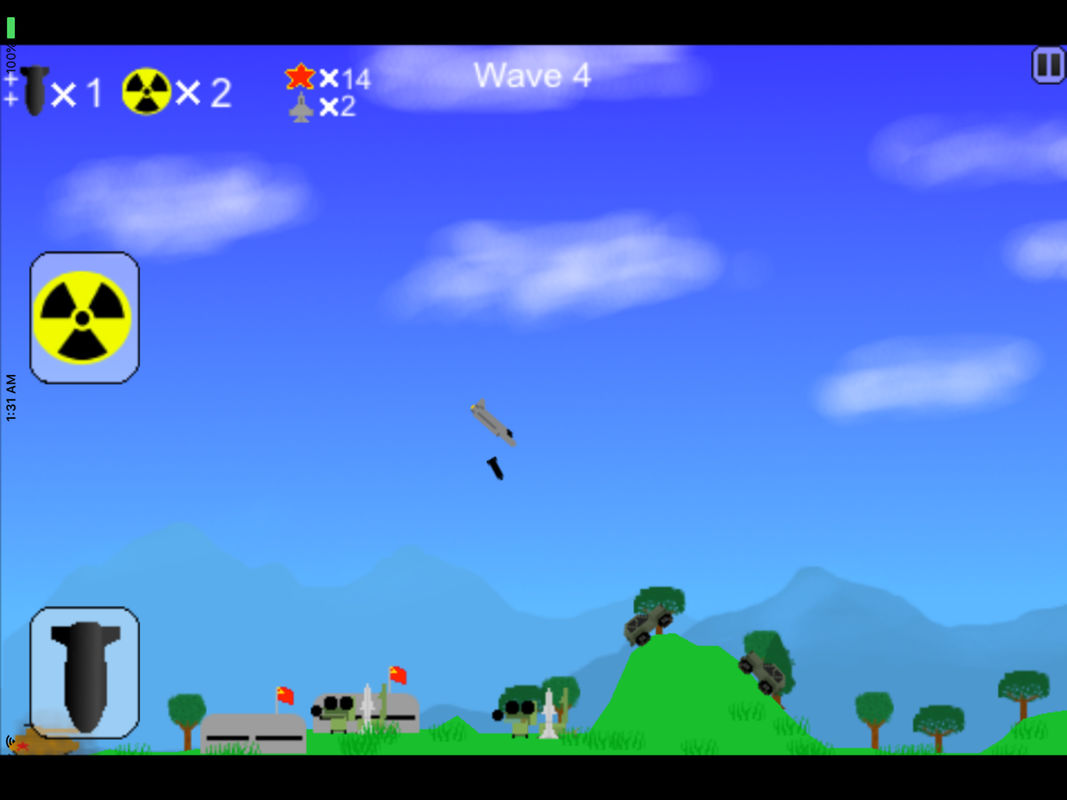
\includegraphics[width=\linewidth]{atomic-bomber}
\caption{Скриншот игрового процесса оригинального <<Atomic Bomber>>}
\end{figure}
\end{section}

\begin{section}{Реализация программы}
\begin{subsection}{Обзор инструментальных средств}
Разработка программы велась на языке C++ в объектно-ориентированной парадигме программирования.
Самостоятельная реализация даже самого базового фреймворка для разработки нашего приложения очень трудоемка, поэтому разработка велась с использованием движка \verb|Urho3D| в качестве фреймворка.
Он предоставляет такие необходимые компоненты как:
\begin{enumerate}
\item Управление жизненным циклом программы, обработка событий ОС.
\item Компонентно-ориентированная модель для описания объектов в 2D/3D среде (сцене), легковесный визуальный редактор сцен.
\item Загрузка текстур и других ассетов в различных форматах, рендеринг 2D и 3D графики, вывод звука, рассчет физики, обработка пользовательского ввода и другие важные подисистемы.
\end{enumerate}

Компонентно-ориентированный подход к построению сцены позволяет удобно реализовывать логику взаимодействия игровых объектов в 2D/3D пространстве и инкапсулировать отдельные ее аспекты.
Его реализация в движке \verb|Urho3D| глубоко интегрирована с объектно-ориентированной парадигмой языка C++ и удачно ее дополняет.

Также была использована библиотека Signals~\cite{signals} в качестве реализации шаблона проектирования <<Observer>>, предоставляющая функционал сигналов и слотов, похожий на делегаты и события в C\#.

Для поддержания качества кода использовались диагностики IDE CLion, а также статический анализ с использованием \verb|PVS-Studio|.
\end{subsection}

\begin{subsection}{Программная реализация}
\begin{subsubsection}{Инициализация}
Входной точкой нашего приложения является класс GameApplication, который регистрируется в движке \verb|Urho3D| макросом \verb|Urho3D_DEFINE_APPLICATION_MAIN(GameApplication)|.
В нем производится получение контекста от \verb|Urho3D|, начальная настройка приложения, вызов регистрации классов компонентов, а также создание и регистрация подсистемы управления игровым состоянием GameSubsystem (в \verb|Urho3D| подсистемами называются объекты, существующие в единственном экземпляре во всем приложении).

GameSubsystem предоставляет функционал загрузки, выгрузки и перезагрузки нашего игрового уровня.
Компоненты на нем, в свою очередь, реагируют на различные события (например, переход на следующий кадр, пользовательский ввод или столкновения), формируя игровой процесс.
\end{subsubsection}

\clearpage
\begin{subsubsection}{Структура уровня}
Уровень (сцена) представляет собой иерархию объектов (называемых Node) и их компонентов:

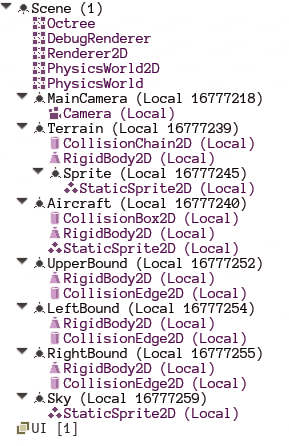
\includegraphics[width=250]{scene}

\begin{enumerate}
\item Объект MainCamera в нашем случае является закрепленной на одном месте ортогональной (не перспективной, т.к. наш мир двухмерен) камерой.
Автоматически масштабируется при запуске для корректного отображения игровой области.
\item Объект Terrain представляет ландшафт.
\item Объект Aircraft представляет самолет игрока.
\item Объект Sky отображает спрайт неба на заднем плане.
\item Объекты LeftBound, RightBound и UpperBound расположены по краям видимой области и содержат физические коллайдеры, не позволяющие игроку покинуть пределы видимого пространства.
\end{enumerate}

Рассмотрим их подробнее.
\end{subsubsection}

\begin{subsubsection}{Ландшафт}
Наиболее комплексная система в нашем приложении, состоит из трех компонентов
\begin{enumerate}
\item \verb|TerrainController| предоставляет логическую модель ландшафта, с которой работают другие компоненты.
\item \verb|TerrainSpriteController| занимается динамической отрисовкой спрайта ландшафта.
\item \verb|TerrainCollisionShapeController| выполняет динамическое построение физической модели ландшафта для работы столкновений.
\end{enumerate}

\verb|TerrainController| содержит карту высот: одномерный массив чисел с плавающей точкой, содержащий высоты в соответствующих точках ландшафта.
Предоставляет методы для деформации ландшафта (взрыва), перевода координат из относительных координат (например, 0.5 будет серединой ландшафта) в абсолютные (мировые), а также событие об изменени ландшафта, позволяющее подписчикам отреагировать на это изменение.

В начале игры карта высот генерируется одномерной версией алгоритма MidpointDisplacement, который рекурсивно генерирует случайную высоту в середине заданного промежутка на основании высот краев:
\clearpage
\inputminted{cpp}{listings/MidpointDisplacement1D.cpp}

При любых изменениях карты высот вызывается событие \verb|HeightmapUpdated|, позволяющее указанным выше компонентам перерисовать спрайт и перестроить сетку коллизий.

\begin{figure}[h]
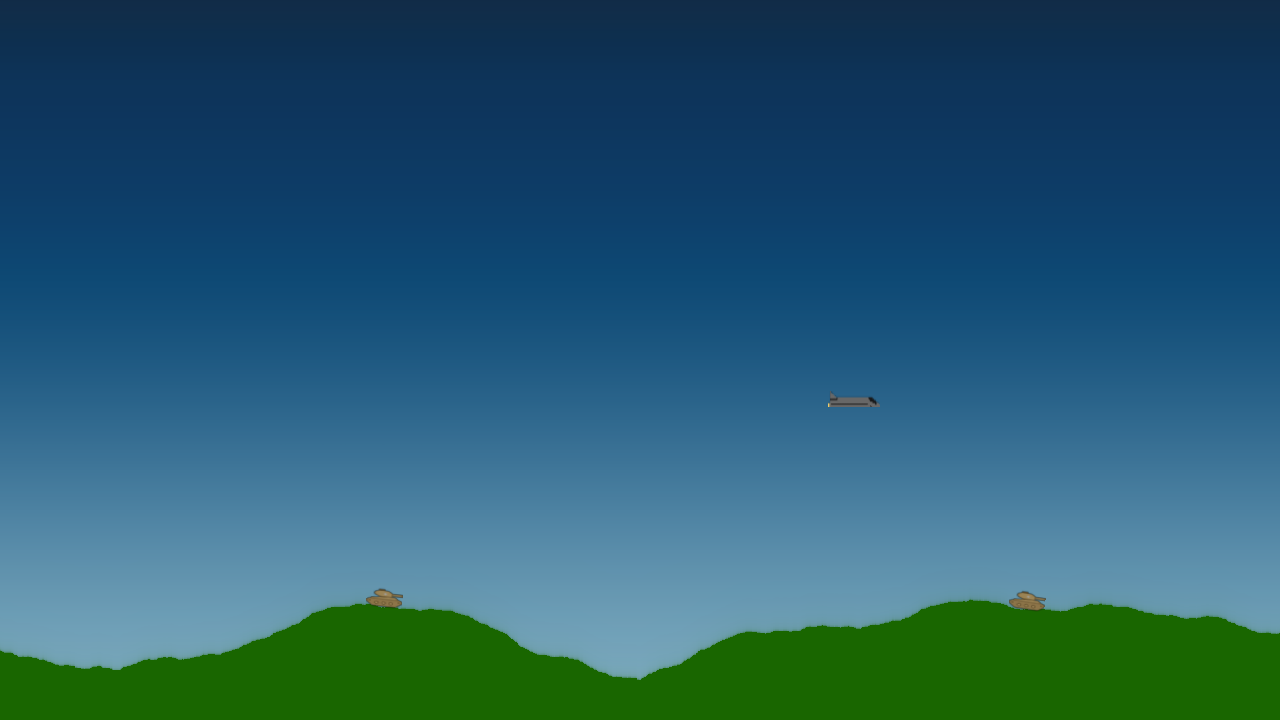
\includegraphics[width=\linewidth]{terrain}
\caption{Пример сгенерированного ландшафта}
\end{figure}
\end{subsubsection}

\begin{subsubsection}{Игрок}
Поведение самолета игрока контроллируют следующие компоненты:
\begin{enumerate}
\item \verb|AircraftController| подписывается на событие столкновения с ландшафтом (для вызова \verb|GameSubsystem::RequestReloadGameLevel| при столкновении), создает остальные компоненты.
\item \verb|AircraftMovingController| контроллирует движение самолета: поддерживает скорость и направление движения, обрабатывает коллизиии с краями мира.
\item \verb|AircraftMouseController| обрабатывает пользовательские клики мышью и отправляет соответствующие команды на изменение направления движения самолета (полет к заданной точке).
\item \verb|AircraftBombsController| обрабатывает нажатие клавиши сброса бомб, инстанцирует объект бомбы.
\end{enumerate}
\end{subsubsection}

\clearpage
\begin{subsubsection}{Коллизии}
Обработка коллизий ведется компонентом \verb|CollisionsAggregator|, который должен быть присутствовать у всех динамических объектов, заинтересованных в регистрации столкновений со статическим окружением.
Оборачивает внутренние физические события \verb|Urho3D| и предоставляет события, соответствующие каждому из типов коллайдеров (описаны далее).
Например, так выглядит подписка самолета на свое столкновение с ландшафтом:

\inputminted{cpp}{listings/AircraftCollisionExample.cpp}

Для того, чтобы была возможность раздельно обрабатывать столкновения с тремя коллайдерами краев мира и ландшафтом, был введен базовый компонент \verb|StaticColliderComponent|, каждый из наследников которого идентифицирует свой тип коллайдера.

Благодаря такому подходу, \verb|CollisionsAggregator| при регистрации столкновения просто проверяет наличие \verb|StaticColliderComponent| на столкнувшемся объекте и проверяет наличие идентификатора его конкретного типа в своем внутреннем словаре подписок.
Если для этого типа коллайдера было создано событие во внутреннем словаре (\verb|HashMap|), то оно будет вызвано.

Выделение этого функционала в универсальный компонент \verb|CollisionsAggregator| позволило избежать дублирования однотипного кода подписок на столкновения в компонентах самолета, бомб и т.д.
\end{subsubsection}

\begin{subsubsection}{Бомбы}
При создании объекта бомбы на ней инициализируется компонент \verb|ShellController|, который в свою очередь обрабатывает движение и столкновения с границами мира, а также инициализирует компонент \verb|ExplosivesController|.
Последний содержит характеристики взрыва и статическое событие \verb|SomethingExploded|, позволяющее таким объектам как ландшафт и противникам отреагировать на взрыв соответствующим образом.
В частности, ландшафт деформируется, а противник будет уничтожен, если находится в радиусе.

Такая событийно-ориентированная организация позволяет в дальнейшем прикрепить этот компонент не только к бомбам, но и к любым другим снарядам, в том числе и направленным против игрока.
Потребуется лишь указать характеристики, а игроку подписаться на событие взрыва.
\end{subsubsection}

\begin{subsubsection}{Противники}
На данный момент представлены только танками.
Структура компонентов практически не отличается от самолета, но вместо контроля игроком выполняется простое движение влево/вправо с заданной скоростью с разворотом у границ мира.
\end{subsubsection}
\end{subsection}

\begin{subsection}{Тестирование}
Проводились тесты на одновременный выброс большого количества бомб, в том числе и в пролете через границу мира.
Также тестировалась многоразовая перезагрузка уровня в разных условиях.

В процессе реализации логики ландшафта была обнаружена и исправлена утечка памяти в используемом внутри \verb|Urho3D| физическом движке \verb|Box2D| (\url{https://github.com/Urho3D/Urho3D/issues/1995}).
Обнаружить и локализовать проблему помог динамический анализатор кода \verb|Valgrind|.

Также регулярно проводились проверки статическим анализатором кода \verb|PVS-Studio|.
\end{subsection}

\end{section}

\begin{section}{Заключение}
В данной курсовой работе удалось реализовать запланированный функционал программы с использованием средства языка C++, а также различных библиотек и инструментов.

Была использована на практике комбинация объектно-ориентированного, компонентно-ориентированного и событийно-ориентированного подходов программирования в совокупности с различными технологиями и инструментами разработки программного обеспечения.

Исходный код проекта и текст данной работы доступны по адресу \url{https://github.com/ArXen42/AlienBomberUrho3D}.
\end{section}

~\nocite{urho3d-docs,cppreference, teplyakov}
\printbibliography[title = Список использованных источников]

\end{document}
